\originalsection{摘要}\label{cat-abstract}
后训练没有真值时，学习信号来自哪里？我们表明，推理计算本身可以充当监督. 通过生成并行采样轨迹并将它们转化为参考估计，模型可以不依赖人类标签而学习；关键是，这甚至适用于医疗指导等不存在程序化检查器的不可验证领域. 我们把框架称为“计算即教师”（Compute as Teacher，CaT），它把并行采样轨迹的推理时计算转化为 RL 训练监督. 框架有两个组件：参考估计把轨迹聚合成伪参考答案，奖励推导把伪参考转化为 RL 奖励. 对前者，我们探索一种称为合成的简单方法，但框架接受任意聚合器；对后者，我们为不可验证领域提出自提出评分细则，即从伪参考生成、由大语言模型判别器计分的二元、可审计标准. HealthBench 上，CaT 训练模型达到或超过推理时聚合质量，而测试时计算减少 9 倍. 在这里，CaT 也可与使用专家医师标注的学习方式竞争，相对初始策略最高改善约 30\%. 框架自然扩展到可验证奖励，在 MATH-500 的测试时 RL 设置下达到最佳已有基线表现，展示跨两类领域的即插即用能力.

\originalsection{1 引言}\paperlabel{1}{cat-sec:introduction}
为获得专门技能而后训练大语言模型，通常依赖带标签参考答案的监督微调\cite{cat-long2022training,cat-wei2022finetuned}，或依赖程序化检查器提供可验证奖励的强化学习. 这种检查器只适用于数学、代码等形式正确性可计算的狭窄领域\cite{cat-lambert2024tulu,cat-shao2024deepseekmath}. 同时，许多有价值任务也没有标注参考答案. 在答案具有定性性质的不可验证场景中，如临床或生活方式指导\cite{cat-arora2025healthbench}、自由对话\cite{cat-roller2020open}和创意写作\cite{cat-paech2023eq}，可能存在多个有效答案，专家可能意见不同，确定性规则检查难以实施. 因而实践者常退回难以扩展的标注流程，或仅靠判别器反馈：让另一大语言模型为自由输出给粗粒度分数，尽管这种方式存在不一致、偏好冗长回答和奖励投机等已知问题.

\begin{figure}[ht]
\centering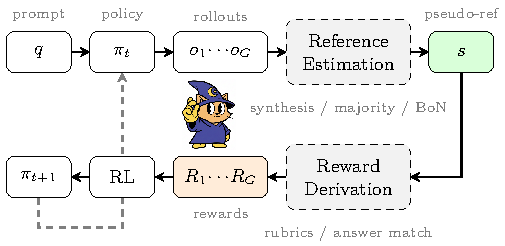
\includegraphics[width=.94\textwidth]{../papers/translations/cat/figures/framework.pdf}
\caption{CaT 框架. 策略 $\pi_t$ 为提示 $q$ 生成 $G$ 条轨迹. 参考估计通过合成、多数投票或 best-of-N，将它们聚合为伪参考 $s$. 奖励推导依据 $s$ 为每条轨迹计分：可验证领域使用答案匹配，不可验证领域使用自提出评分细则. 奖励驱动 RL，更新策略. 原图：Dulhan Jayalath 等，完整作者名单见文首，CC BY 4.0；由原作者 TikZ 导出，英文标注保留.}\label{cat-fig:framework}
\end{figure}
本文转而提出一个简单问题：\emph{推理计算能否替代缺失的监督？}

\textbf{计算即教师.} 我们回答“能”. CaT 用参考估计和奖励推导两个组件，把推理计算转成监督. 关键是，并行轨迹对模型的不确定性进行采样，因为它们恰好在模型不确定之处分歧. 一条轨迹可能有正确中间步骤，另一条有正确最终答案，第三条有有用验证；总体集合比单条包含更多信息. 参考估计把分散信息聚合为一个伪参考，奖励推导依据它为轨迹计分，以用于 RL. 框架不依赖具体聚合方法：多数投票、best-of-N 等选择策略找回最佳轨迹，生成策略则组合各轨迹片段，构建新回答. 我们探索简单的合成策略，让冻结策略条件于轨迹集合构建新回答，但任意聚合器都可接入同一奖励推导机制. GRPO 等组式 RL 已经为优势估计生成并行轨迹，因此参考估计增加的开销很小.

\textbf{不可验证领域的无参考奖励.} 奖励推导因领域而异. 数学、代码等可验证场景中，简单检查轨迹答案是否与伪参考一致. 更难的是没有这种检查的不可验证领域. 我们提出另一项关键贡献——自提出评分细则，让模型生成刻画伪参考的二元标准，如“建议咨询医疗专业人员”“指出患者对心律失常的担忧”. 独立大语言模型判别器逐项检查，奖励为满足标准的比例. 由此，不依赖真值也能为每条轨迹给奖励，在不可验证领域进行无参考 RL.

\textbf{有效原因的直观解释.} 轨迹从模型不确定性采样，分歧揭示了模型犹疑之处. 合成迫使模型检查分歧，依据证据选择一个观点或构建调和方案；选择方法只能挑一个已有答案. 不可验证领域的细则问“回答是否满足标准 X”，而非“回答好不好”；分解把模糊判断变成细粒度二元检查的求和，使验证更容易. 关键是，从伪参考自提出细则后，CaT 无需任何人类标注参考答案，就能为不可验证领域的轨迹提供奖励.

\textbf{实用性.} 框架实用且即插即用，无需人类标签、领域专用验证器，并复用标准 RL 已花费的组采样计算. CaT 把推理时聚合的收益摊入模型权重，在达到或超过聚合表现的同时，把每次查询的测试时计算最多减少 9 倍. 训练后策略回答质量还常超过初始聚合伪参考，并持续改进，直到轨迹趋于相似回答. 我们在 Gemma 3 4B、Qwen 3 4B、Llama 3.1 8B 三个模型家族，以及不可验证 HealthBench 和可验证 MATH-500 上验证.

\textbf{CaT 连接多条研究路线.} 它像自训练\cite{cat-schmidhuber2003exploring,cat-schmidhuber2013powerplay,cat-silver2016mastering,cat-silver2018general}和知识蒸馏\cite{cat-hinton2015distilling}一样，从模型生成监督学习，但通过调和多个样本产生目标，而非信任单个自标签. 它像多数投票、best-of-N 等测试时扩展方法一样利用并行轨迹，但通过 RL 把改善摊入权重. 相比大语言模型充当判别器的奖励\cite{cat-zheng2023judging}，细则评分提供分解、具体的标准，缓解不稳定和偏见\cite{cat-dineen2025qa,cat-gunjal2025rubrics}. 最后，CaT 把学习扩展到没有形式检查器的领域，补充程序化验证\cite{cat-lambert2024tulu}.

\textbf{贡献：}
\begin{enumerate}
\item 不可验证 RL 的自提出评分细则：将判断分解为二元标准的奖励机制，让没有程序化检查器的领域也能进行无参考 RL.
\item 计算即教师：通过参考估计和奖励推导，把推理计算转成监督的一般范式，合成是其中一种有效参考估计器.
\item 全面经验研究：三个模型在 HealthBench 与 MATH-500 上取得增益，训练模型用少 9 倍计算达到或超过推理时质量.
\end{enumerate}
\textbf{文章安排.} 第\ref{cat-sec:relatedwork}节讨论相关工作；第\ref{cat-sec:method}节形式化框架和自提出细则；第\ref{cat-sec:experiments}节给出实验设置；第\ref{cat-subsec:main-results}节给出结果、消融与分析；第\ref{cat-sec:discussion}节讨论局限、未来方向并总结.

\originalsection{2 相关工作}\paperlabel{2}{cat-sec:relatedwork}
\textbf{无参考微调.} 自生成监督在大语言模型训练中历史悠久. Constitutional AI\cite{cat-bai2022constitutional}用自我修订的生成结果训练，Self-Instruct\cite{cat-wang2023selfinstruct}生成并筛选自身的指令遵循数据，Quiet-STaR\cite{cat-zelikman2024quiet}在没有参考轨迹时学习产生推理 token. 它们针对无害性、指令遵循和推理等专门能力. CaT 更一般：只要模型能生成多样轨迹，且不可验证领域中的细则判断可靠，就支持无人工参考的 RL.

\textbf{无参考 RL.} 近期工作探索无真值标签的 RL. TTRL\cite{cat-zuo2025ttrl}用多数投票共识作数学伪标签，Absolute Zero\cite{cat-zhao2025absolute}在自行提出的数学和代码问题上自博弈. 这些方法有效，但局限于正确性可由程序检查的领域. 另一条路线最小化熵或最大化自确定性\cite{cat-zhao2025learning,cat-agarwal2025unreasonable,cat-prabhudesai2025maximizing,cat-gao2025one,cat-li2025confidence}. Wen 等\cite{cat-wen2025unsupervised}依据互可预测性为多项选择答案评分. 这些方法具有判别性质，只选择或评分已有输出. CaT 可用任一方法作参考估计器，也能超越选择；如果采用合成，它可构建采样集合分布之外的伪参考. 更重要的是，CaT 通过自提出细则扩展到不可验证领域，先前方法尚未用于这种设置；我们将其改为基线时，表现不及 CaT（第\ref{cat-subsec:ref-estimation}节）.

\textbf{测试时扩展.} 并行轨迹长期用于改善推理表现. 多数投票或自一致性\cite{cat-wang2023}选最常见答案；best-of-N 依信心、困惑度或大语言模型判断选择\cite{cat-zheng2023judging}. 它们提升准确率，却不把收益写入权重，每次部署都承担完整 $G$ 条轨迹成本. CaT 用同样轨迹生成 RL 监督，把推理计算摊入训练. 训练后模型以 $1/G$ 测试时成本达到或超过聚合质量，因此大部分计算在训练中一次性花费，而非推理时反复支付.

\textbf{不可验证 RL.} 无法程序化验证时如何产生奖励？已有方法假定可访问参考答案. VeriFree\cite{cat-zhou2025reinforcing}、JEPO\cite{cat-tang2025beyond}和 RLPR\cite{cat-yu2025rlpr}计算参考答案在模型推理链条件下的概率. Rubrics as Rewards（RaR）\cite{cat-gunjal2025rubrics}从参考答案构建评价细则，再由大语言模型判断评分，展示细则奖励优于直接评分. 我们继承此认识，但完全消除参考依赖：CaT 从轨迹估计的伪参考自提出细则. 推理计算生成伪参考，伪参考生成细则，细则生成奖励；流程没有人类标注进入.

\originalsection{3 计算即教师}\paperlabel{3}{cat-sec:method}
CaT 通过参考估计和奖励推导两个组件将推理计算转为监督，图\ref{cat-fig:framework}展示框架. 给定提示 $q$，当前策略 $\pi_t$ 生成 $G$ 条并行轨迹 $o_{1:G}$. 它们在模型不确定之处不同，因而采样其不确定性. 参考估计聚合为单个伪参考回答 $s$，用作监督目标. 奖励推导依据 $s$ 为每条 $o_i$ 产生 RL 奖励 $R(o_i;s)$.

框架不依赖具体聚合方法. 多数投票和 best-of-N 从已有轨迹选一个 $s$；合成等生成策略条件于全部轨迹构建新的 $s$，可能组合分散在集合中的正确片段. 本文经验探索合成，但奖励推导机制，尤其不可验证领域的自提出细则，可以配合任意参考估计策略.

\textbf{记号.} $q$ 为提示，$o_i$ 为采样轨迹，$s$ 为伪参考，$\mathcal R=\{r_j\}$ 为由二元标准组成的细则，$\pi_t$ 为第 $t$ 步当前策略，$\pi_0$ 为冻结锚点即初始策略，$\pi_J$ 为细则计分的判别模型.

\subsection*{3.1 参考估计}\paperlabel{3.1}{cat-subsec:ref-estimation}
参考估计把 $G$ 条轨迹聚合成一个伪参考 $s$，任意聚合策略均兼容，包括：
\begin{itemize}
\item 多数投票：$s$ 为 $o_{1:G}$ 中最常见的最终答案\cite{cat-zuo2025ttrl}，只适用于可比较答案的可验证领域.
\item Best-of-N：对某评分函数 $f$，令 $s=\arg\max_{o_i}f(o_i)$；可使用模型困惑度\cite{cat-agarwal2025unreasonable}、信心启发式\cite{cat-li2025confidence}或判别器分数.
\item 合成：冻结锚点 $\pi_0$ 条件于轨迹集合，按某提示生成新回答，调和其中的信息.
\end{itemize}
选择最多找回最佳轨迹. 合成可构建组合多个正确片段的回答，潜在地超过全部轨迹. 我们聚焦合成，并在第\ref{cat-subsec:synthesis-results}节与选择基线比较.

\textbf{合成.} 给定 $o_{1:G}\sim\pi_t(\cdot\mid q)$，锚点生成
\begin{equation}
s\sim\pi_0(\cdot\mid p_{\mathrm{syn}},o_{1:G}).\label{cat-eq:synthesis}
\end{equation}
$p_{\mathrm{syn}}$ 指示模型将轨迹调和成一个更好的回答；完整提示见附录\hyperref[cat-app:prompts]{F}. 两个设计选择值得解释. 第一，为简便，我们从锚点输入中省去原提示 $q$，消融见附录\hyperref[cat-app:omittingq]{A.4}. 第二，使用冻结初始策略而非当前策略，使探索与估计解耦：$\pi_t$ 经 RL 探索改进，$\pi_0$ 提供参考估计，只优化 $\pi_t$.

\textbf{合成何时有帮助？} 轨迹在模型犹疑之处分歧. 一条可能有正确中间步骤但结论错误，另一条可能通过有缺陷推理得到正确答案. 合成检查分歧，整合互补证据，如一条的正确步骤和另一条的有效检查. 实验中，合成在 5--15\% 问题上不同于多数答案，也可不同于全部轨迹却仍正确（第\ref{cat-subsec:analysis}节）. 这提示它进行某种结构化生成调和，而非只改写答案并充当选择器.

\subsection*{3.2 奖励推导}\paperlabel{3.2}{cat-subsec:reward-derivation}
给定伪参考 $s$，为 RL 导出每条轨迹的奖励，机制依领域而异.

\Needspace{5\baselineskip}
\noindent\textbf{3.2.1 可验证领域}\phantomsection\label{cat-subsubsec:verifiable}\par
正确性可以程序检查时，奖励与伪参考一致：
\begin{equation}
R_{\mathrm{ver}}(o;s)=\mathbf1[\texttt{answer}(o)=\texttt{answer}(s)].\label{cat-eq:verifiable}
\end{equation}
数学问题中，\texttt{answer} 提取最终方框表达式，再检查字符串等价. 这有意保持简单，因为此领域的复杂性在参考估计而非奖励推导.

\Needspace{5\baselineskip}
\noindent\textbf{3.2.2 不可验证领域}\phantomsection\label{cat-subsubsec:nonverifiable}\par
同等优质答案可有大量表达方式，规则方法不实用，因此没有这种检查器. 直接让大语言模型打 1--10 分等朴素替代方案，存在提示间不一致、偏好冗长或流畅风格、易受奖励投机影响等已充分记录的问题\cite{cat-zheng2023judging,cat-arora2025healthbench}. 我们改为将判断分解成从伪参考生成、分别计分的自提出二元细则（图\ref{cat-fig:rubric}）.

\textbf{生成细则.} 锚点依据伪参考生成 $\mathcal R=\{r_1,\ldots,r_n\}$：
\begin{equation}
\mathcal R\sim\pi_0(\cdot\mid p_{\mathrm{rub}},s).\label{cat-eq:rubric-gen}
\end{equation}
每个 $r_j$ 是刻画 $s$ 重要属性的二元、可验证陈述. 提示要求至少 5 条具体标准，完整生成提示见附录\hyperref[cat-app:prompts]{F}.

\textbf{细则计分.} 独立判别模型 $\pi_J$ 检查轨迹是否满足每条标准：
\begin{equation}
R_{\mathrm{rub}}(o;\mathcal R)=\frac1n\sum_{j=1}^n\mathbf1[\pi_J(o,r_j)=\text{``yes''}].\label{cat-eq:rubric-reward}
\end{equation}
奖励为按判别器判断满足标准的比例.

\textbf{为何用细则？} 分解有三个优点：可靠性——“是否建议专业咨询”比“回答好不好”更容易一致地判断；可审计性——可查看满足或失败的标准，便于调试分析，而直接分数不透明；减轻表面形式偏差——无论措辞、长度、格式如何，都可满足“建议改变生活方式”，因此有助于奖励内容而非风格.

\textbf{例子.} 用户询问轻度高血压管理，合成产生建议饮食改变、运动与医疗随访的伪参考，锚点生成细则：承认用户所述症状；建议饮食、运动等生活方式改变；建议咨询医疗服务提供者；避免确定性诊断；语气有同理心且适当. 若轨迹满足第 1、2、3、5 项而不满足第 4 项，则得 $R=4/5=0.8$.
\begin{figure}[ht]
\centering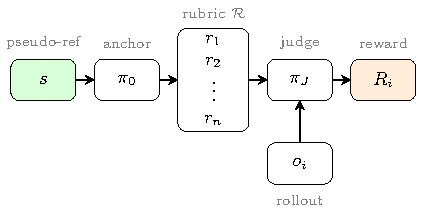
\includegraphics[width=.84\textwidth]{../papers/translations/cat/figures/rubric.pdf}
\caption{不可验证领域基于细则的奖励. 锚点 $\pi_0$ 从伪参考 $s$ 生成二元是／否标准 $\mathcal R=\{r_1,\ldots,r_n\}$. 判别器逐项为轨迹 $o_i$ 计分，奖励为满足的比例. 原图：Dulhan Jayalath 等，完整名单见文首，CC BY 4.0；由原作者 TikZ 导出，英文标注保留.}\label{cat-fig:rubric}
\end{figure}

\subsection*{3.3 训练}\paperlabel{3.3}{cat-subsec:training}
我们用组相对策略优化 GRPO\cite{cat-shao2024deepseekmath}实现 CaT，但奖励形式兼容每个提示采样多条轨迹的任意策略梯度方法. 每个提示采样 $G$ 条轨迹，以组均值计算优势：
\begin{equation}
\widehat A_i=\frac{R(o_i;s)-\overline R_G}{\sigma_G}.\label{cat-eq:advantage}
\end{equation}
其中 $\overline R_G=G^{-1}\sum_jR(o_j;s)$，$\sigma_G$ 为标准差. 策略通过带截断和相对初始策略 KL 正则的替代目标更新，细节见附录\hyperref[cat-app:grpo]{E}.

GRPO 已为优势估计生成 $G$ 条轨迹，CaT 复用它们，只增加一次合成调用以生成 $s$；不可验证领域另加一次细则生成调用，再进行 $nG$ 次判别调用. 合成调用成本相当于多生成一条轨迹；$nG$ 次判别可并行，输出只有是／否等很少 token，费用较低. 实际上，相比生成 $G$ 条轨迹，参考估计和奖励推导只增加适度开销.

\textbf{训练循环.} 下列算法概括一次迭代：采样、估计伪参考、导出奖励，再用 GRPO 更新.
\phantomsection\label{cat-alg:cat-rl}
\noindent\textbf{原文算法 1：CaT 的一次训练步骤}
\begin{enumerate}
\item 输入：当前策略 $\pi_t$、锚点 $\pi_0$、判别器 $\pi_J$、提示 $q$、参考估计器 Aggregate.
\item 采样 $o_{1:G}\sim\pi_t(\cdot\mid q)$；估计 $s\leftarrow\mathrm{Aggregate}(o_{1:G})$，例如合成或多数投票.
\item 若 $q$ 可验证，对每个 $i=1,\ldots,G$，令 $R_i\leftarrow\mathbf1[\texttt{answer}(o_i)=\texttt{answer}(s)]$.
\item 否则，生成 $\mathcal R\sim\pi_0(\cdot\mid p_{\mathrm{rub}},s)$；对每个 $i$，令 $R_i\leftarrow|\mathcal R|^{-1}\sum_{r\in\mathcal R}\mathbf1[\pi_J(o_i,r)=\text{``yes''}]$.
\item 计算 $\widehat A_i=(R_i-\overline R_G)/\sigma_G$；用 $\{(o_i,\widehat A_i)\}_{i=1}^G$ 经 GRPO 更新策略.
\end{enumerate}

\textbf{推理时使用.} 参考估计也可仅用于推理、不训练 RL. 从初始策略为提示生成 $G$ 条轨迹，估计伪参考并返回它. 这以至少 $G$ 倍推理计算带来即时准确率收益，但没有转入权重，每次部署都付全额成本. CaT 将收益摊入训练，训练后策略只产生一个输出，就可达到相似或更好质量. 实验中，它以少 9 倍测试时计算达到或超过推理时合成.

\originalsection{4 实验}\paperlabel{4}{cat-sec:experiments}
我们主要评价以合成作为参考估计的 CaT 训练框架，其次单独评价不训练时的合成，隔离各组件收益. 实验回答：CaT 能否改进初始策略，并以更低测试成本达到或超过推理时合成？自提出细则能否在不可验证领域提供有效奖励？合成与选择基线的参考估计相比如何？

\subsection*{4.1 设置}\paperlabel{4.1}{cat-subsec:setup}
\textbf{数据集.} HealthBench\cite{cat-arora2025healthbench}含医师与用户的 5000 段自由医疗对话，是有多个有效定性答案、无程序检查器的不可验证领域. 留出 500 段有医师设计评价细则的对话测试，其余用于无参考训练与验证. MATH-500\cite{cat-hendrycks2021measuring}含 500 道竞赛数学题，最终答案可程序检查. 遵循 TTRL\cite{cat-zuo2025ttrl}，在同一 500 题上训练测试，训练不访问任何参考标签，属于测试时训练设置. HealthBench 是主要试验场，因为不可验证领域是更困难、尚未解决的问题；MATH-500 展示框架无需修改可跨领域类型泛化，是统一即插即用框架，而非不可验证领域专用方法.

\textbf{模型.} 评价三个 4--8B 规模指令调优模型家族：Gemma 3 4B Instruct\cite{cat-team2025gemma}、Qwen 3 4B Instruct\cite{cat-yang2025qwen3}和 Llama 3.1 8B Instruct\cite{cat-grattafiori2024llama}. 合成与细则生成的锚点均为训练前初始策略；细则计分使用 GPT-4o\cite{cat-hurst2024gpt}作为判别器. 除非另有说明，CaT 的参考估计始终使用合成.

\textbf{评价.} HealthBench 按留出医师细则报告回答准确率，并如基准论文一样由 GPT-4o 计分. MATH-500 报告最终答案正确比例. 始终取 $G=8$. 误差棒是跨测试样本计算的标准误. 超参数和更多细节见附录\hyperref[cat-app:hparams]{H}、\hyperref[cat-app:expdetails]{I}.

\subsection*{4.2 主要结果}\paperlabel{4.2}{cat-subsec:main-results}
图\ref{cat-fig:headline}概括主要发现. 所有模型与两个领域中，CaT 均改进初始策略；相对未训练策略，HealthBench 最高改善约 30\%，MATH-500 约 33\%.

\textbf{达到或超过推理时合成.} HealthBench 上 CaT 一致优于推理时合成. MATH-500 二者相近，Gemma 和 Llama 中 CaT 稍好，Qwen 中稍差. 关键是，在 HealthBench 的泛化归纳设置中，CaT 用少 9 倍测试时计算达到这种表现：训练策略只产生一个回答，推理时合成要 8 条轨迹加一次生成.

\textbf{改进持续到轨迹收敛.} 更好策略生成信息更丰富轨迹，产生更好伪参考，进一步改进策略. 全部模型中观察到这一动态：6 个模型—数据集对中，5 个超过自己的教师信号，即初始合成伪参考. 足够训练后，轨迹趋于一致，留给合成调和的分歧减少，伪参考相对单条轨迹的增量信号递减（附录\hyperref[cat-app:catrl-stops-learning]{D}）. 这与 RL 微调中已知的熵坍缩一致\cite{cat-yue2025does,cat-song2025mind}.
\begin{figure}[ht]
\centering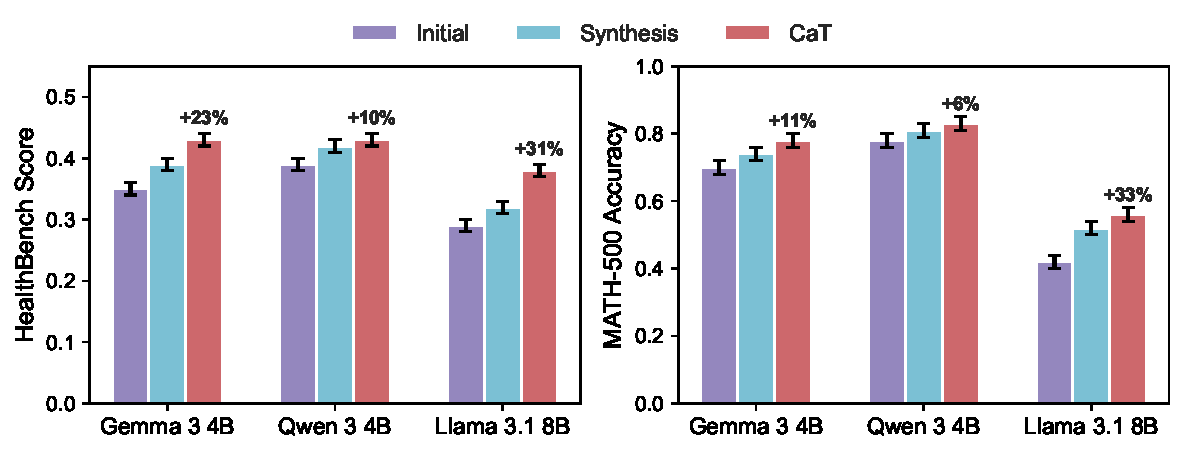
\includegraphics[width=.94\textwidth]{../papers/translations/cat/figures/cat_comparison.pdf}
\caption{CaT 相对初始策略最多改善 30\%. 它以少 9 倍测试时计算达到或超过推理时合成. 在 HealthBench 上，Gemma 和 Llama 的 CaT 优于合成，Welch $t$ 检验 $p<0.05$. 原图：Dulhan Jayalath 等，CC BY 4.0；英文标注保留.}\label{cat-fig:headline}
\end{figure}

\subsection*{4.3 不可验证领域的自提出细则}\paperlabel{4.3}{cat-subsec:rubric-results}
核心挑战是奖励推导，因此比较：从伪参考生成的自提出细则、HealthBench 人工标注医师细则这一理想基线，以及直接由大语言模型判断轨迹是否匹配伪参考的模型直接评判.

图\ref{cat-fig:rubric-comparison}左显示，自提出细则在三个模型上均优于模型直接评判，在其中两个上与医师细则相近. 无人工输入时，模型生成的评价标准有时与专家设计一样有效. 粗粒度判断脆弱可能解释直接评判表现较差. 图右比较 CaT 与在合成伪参考上监督微调的 CaT-SFT. CaT 在全部模型上获胜，常有明显差距，如 Llama 的 0.38 对 0.28. 这与有限数据下 RL 比 SFT 更好泛化的先前发现一致\cite{cat-chu2025sft,cat-gunjal2025rubrics}.
\begin{figure}[ht]
\centering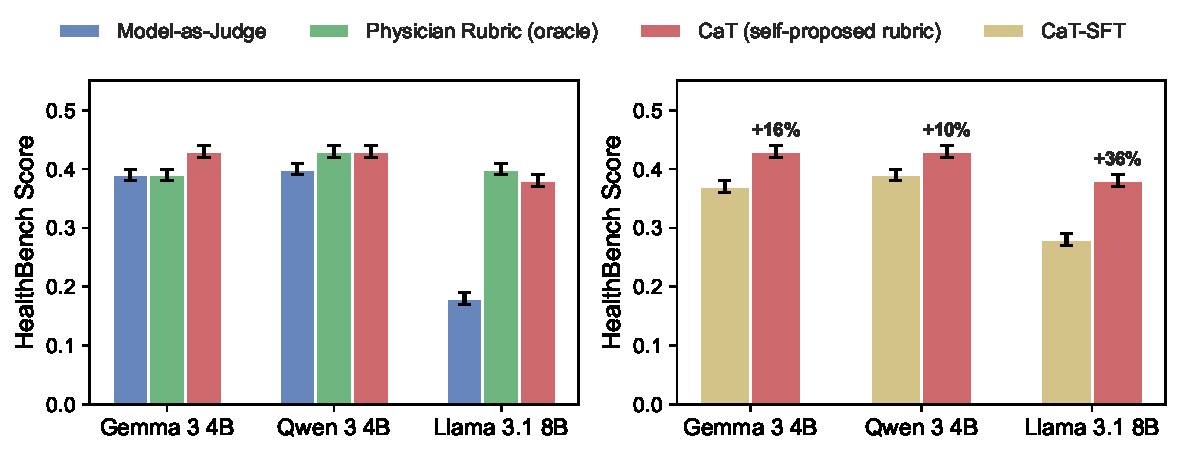
\includegraphics[width=.94\textwidth]{../papers/translations/cat/figures/healthbench_ablation.pdf}
\caption{左：自提出细则可比于医师细则，并优于模型直接评判（$p<0.05$）. 右：基于细则奖励的 RL 优于在合成参考上 SFT. CaT 在所有情形均优于 CaT-SFT（$p<0.05$）. 显著性用 Welch $t$ 检验. 原图：Dulhan Jayalath 等，CC BY 4.0；英文标注保留.}\label{cat-fig:rubric-comparison}
\end{figure}

\subsection*{4.4 参考估计：合成与选择}\paperlabel{4.4}{cat-subsec:synthesis-results}
在不训练 RL 的推理时比较合成与选择基线，以识别适合框架的参考估计策略. 基线包括：单样本；在 $G$ 条轨迹中选最常见最终答案的多数投票，仅可验证领域使用；策略选择自身最佳回答的 Self-BoN；最低困惑度选择\cite{cat-agarwal2025unreasonable}；以及互可预测性\cite{cat-wen2025unsupervised}，即选择条件于其他全部轨迹时概率最高的回答.

图\ref{cat-fig:inference-comparison}显示各模型与数据集的推理表现. 合成在不可验证 HealthBench 上优于全部基线，在 MATH-500 上也达到或超过它们，支持跨类型直接使用. 附录\hyperref[cat-app:rlcomp]{A.1}还给出其他选择方法的部分 RL 结果. 最老的 Llama 3.1 8B 相对选择的合成收益较小，却有最大 RL 收益. 合成要求识别并解决轨迹差异，较弱模型可能因元认知推理基础能力较低而困难.
\begin{figure}[ht]
\centering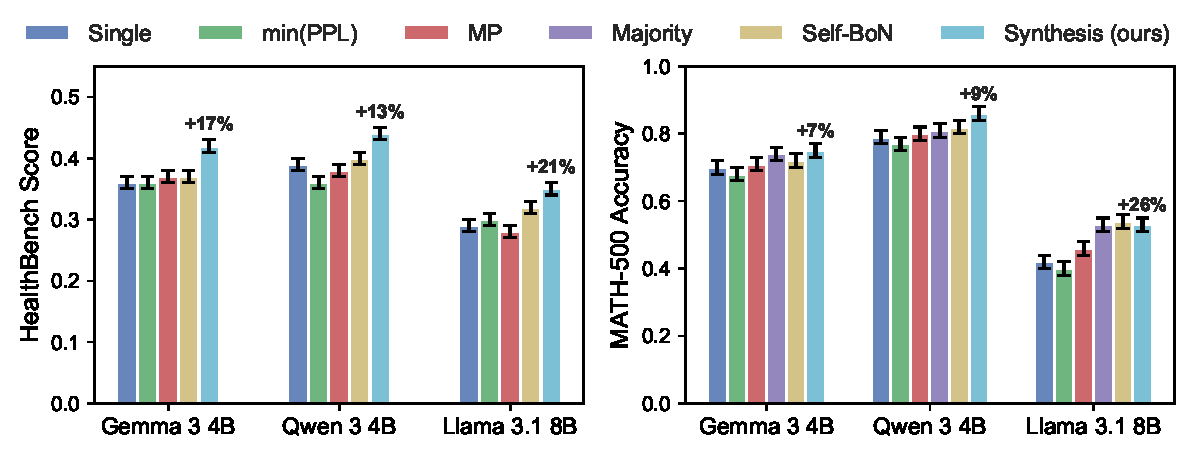
\includegraphics[width=.94\textwidth]{../papers/translations/cat/figures/inference_methods_comparison.pdf}
\caption{不可验证 HealthBench 上，合成在推理时超过选择基线. 可验证 MATH-500 上也能与最佳方法竞争，支持跨领域即插即用. 改善百分比相对单样本. HealthBench 上相对次佳方法的全部合成增益，都经 Welch $t$ 检验达到 $p<0.05$. 原图：Dulhan Jayalath 等，CC BY 4.0；英文标注保留.}\label{cat-fig:inference-comparison}
\end{figure}

\subsection*{4.5 合成与选择有何不同}\paperlabel{4.5}{cat-subsec:analysis}
选择最多找回最佳轨迹，合成等生成方法可构建潜在超过最佳轨迹的新回答. 本节分析何时、如何体现这一差别.

表\ref{cat-tab:disagreement}显示，合成在 5--7\% 问题上与多数投票不同，在 7--10\% 上与 Self-BoN 不同. 不同之处的正确率显著高于机会水平：相对多数投票为 82--86\%，相对 Self-BoN 为 70--82\%. 因此分歧平均提供改善表现的答案，超出选择方法所能触及的范围.

约 1\% 的问题中，全部轨迹错误而合成产生正确答案. 选择不可能做到，因为答案在采样集合分布之外. 附录\hyperref[cat-app:disagree]{B}给出互补算术错误的实例，合成整合正确推理步骤同时避免错误.

也可能怀疑合成只受益于额外生成一个样本，而未使用轨迹. 为检验这一点，在 Qwen 3 4B、MATH-500 上比较条件于 8 条与 1 条轨迹：单轨迹上下文时，仅从 0.79 小幅改善到 0.80；8 条时，明显优于多数投票，0.85 对 0.81. 因而合成可能调和跨轨迹信息，而非充当独立样本. 附录\hyperref[cat-app:analysis]{C}对输出的分析提供进一步证据.
\begin{longtable}{lcc}
\caption{合成可能与选择方法不一致，并在不一致时给出正确答案. MATH-500 上 7 个种子的平均结果；平均而言，这些分歧有助于改进.}\label{cat-tab:disagreement}\\

        \toprule
        \textbf{比较} & $p$(不一致) & $p$(正确 $\mid$ 不一致) \\
        \midrule
        \multicolumn{3}{l}{\textit{Qwen 3 4B}} \\
        Synth. vs Maj. vote & $4.8\%$ & $\mathbf{86.3\%}$ \\
        Synth. vs Self-BoN & $6.5\%$ & $\mathbf{81.7\%}$ \\
        \midrule
        \multicolumn{3}{l}{\textit{Gemma 3 4B}} \\
        Synth. vs Maj. vote & $7.4\%$ & $\mathbf{81.5\%}$ \\
        Synth. vs Self-BoN & $9.9\%$ & $\mathbf{70.2\%}$ \\
        \bottomrule
    
\end{longtable}


\originalsection{5 讨论}\paperlabel{5}{cat-sec:discussion}
\textbf{局限与未来工作.} CaT 要求初始模型能生成有用轨迹，并在使用合成时连贯地调和它们；基础表现较低的模型收益较小. 框架继承 RL 的已知限制：策略改善时轨迹多样性减少，合成可调和的分歧变少，轨迹收敛后增益进入平台期. 表现还可能依赖判别器能力（附录\hyperref[cat-app:judge-sens]{A.3}）. 未来可通过更好采样或探索奖励\cite{cat-song2025outcome}生成更多样轨迹. 参考估计和奖励推导可独立改进：学习的聚合器可能优于提示式合成；部分得分、层级标准、信心加权等细粒度细则可能提高评分准确性与粒度. 除单轮回答，还可扩展到推理轨迹、多轮对话或智能体行动轨迹.

\textbf{结论.} 我们提出把推理计算转为监督的 CaT. 并行轨迹采样模型不确定性，参考估计聚合为伪参考，奖励推导转为 RL 奖励. 框架不依赖聚合方式，合成是一种强选项，多数投票与 best-of-N 也可用. 核心贡献是在不可验证领域支持无参考 RL：自提出细则无需人工标注提供稳定奖励. HealthBench 上，细则表现相近于医师设计，CaT 相对初始策略最多改善 30\%，训练模型以少 9 倍测试时计算达到或超过聚合质量. 因而计算可在训练中花一次，替代推理中反复支付. 可验证 MATH-500 上表现与其他方法一样好，展示跨类型即插即用. 当参考答案稀少、昂贵、有争议甚至未知时，CaT 提供实用后训练框架. 人工标注成为专门领域瓶颈时，从推理计算学习提供了一条可能的路径.

\originalsection{致谢}\label{cat-acknowledgements}
按姓名字母顺序，我们感谢 Joseph Brennan 协助处理细则数据，Lovish Madaan 提供多种技术帮助，Nicola Cancedda 对机构审批流程给予反馈，Stéphane Collot 指导细则生成，Yonatan Gideoni 评论本文草稿，以及 Yunzhen Feng 提供一般技术建议. DJ 在本研究时是 Meta 实习生，并得到 EPSRC Autonomous Intelligent Machines and Systems（AIMS）博士训练中心的 AWS Studentship 支持，项目号 EP/S024050/1.
